\label{chap_transport}

Based on the volume fraction of dispersed phases, numerical simulation of two-phase flow can be defined into the following models:

\begin{itemize}
  \item {Interface tracking model (IT)}, 
  \item {Eulerian-Eulerian model (E-E)}, 
  \item {Lagrangian particle tracking model (LPT)},
  \item {Lattice Boltzmann Method(LBM), etc}.
\end{itemize}

%\subsection{Results and footer outputtttttttttttttt} 

%Results, plotted from lines~114--116 (not shown here) are displayed in Fig.~\ref{fig_approaches}.

%--------------%
%              %
%  Approaches  %
%              %
%--------------%
\begin{figure}[ht]
  \centering
  \setlength{\unitlength}{ 1mm}
  \begin{picture}( 250, 80)( 0, 0)
    \thickbox{ 250}{ 80}
    \put( 25, 0){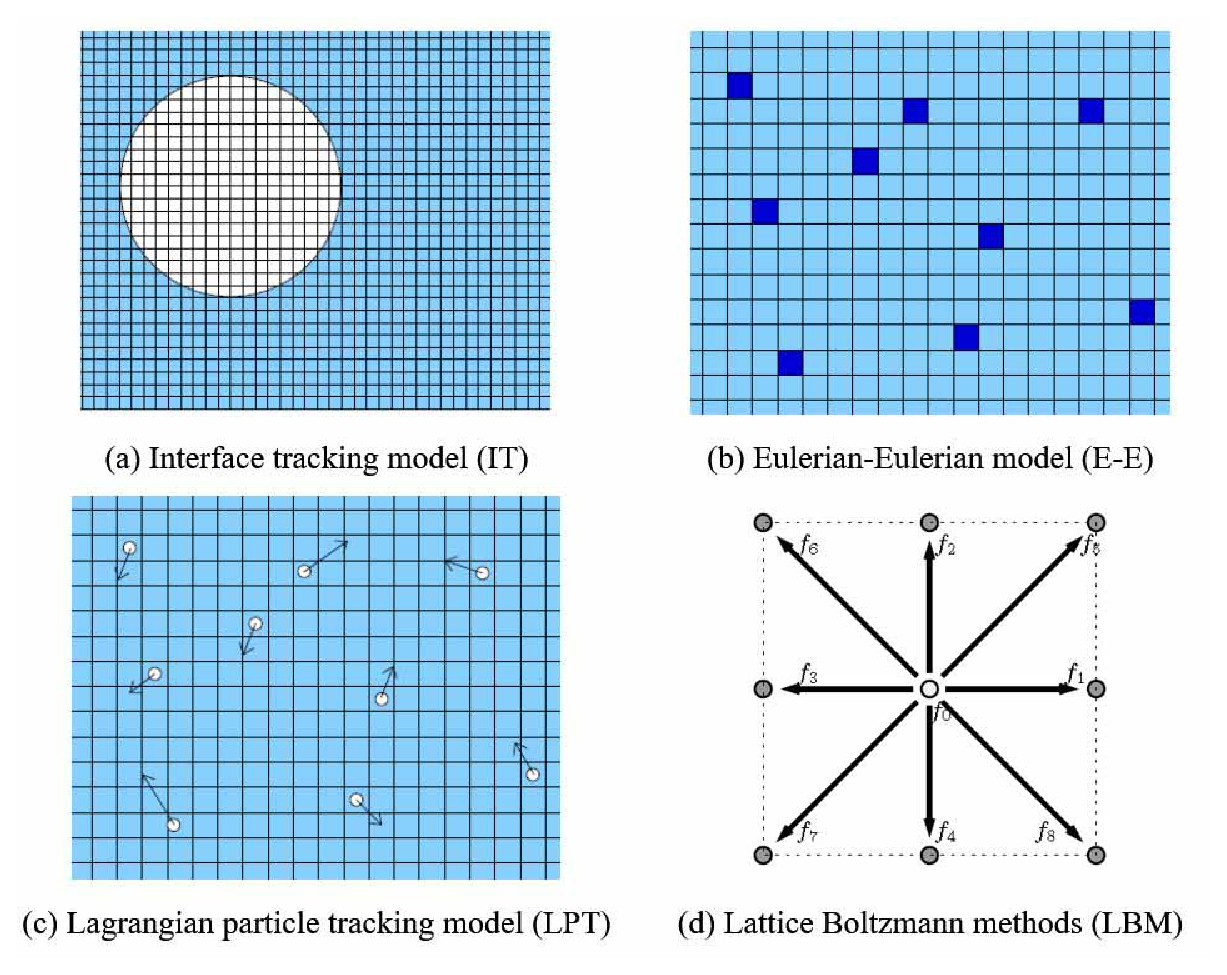
\includegraphics[scale=0.50]{Figures/10-LPT/10-01-approaches.eps}}
  \end{picture}
  \caption{Different approaches to simulate various types of multiphase flows.}
  \label{fig_approaches}
\end{figure}

The rational constrained interpolation profile (R-CIP) with the conservative semi-Lagrangian (CSL2) scheme coupled with local sharpening (CIPCSL2)\footnote{\tt Sato, Y. and Niceno, B. A conservative local interface sharpening scheme for the constrained interpolation profilemethod. Int. J. Numer.Methods Fluids, 70:441–467, 2012.} is used in {\psiboil} for interface tracking (IT).

The main challenges of IT approaches are in advancing the interface accurately with proper implementation of boundary conditions such as surface tension force.  The main drawback is the high computational cost since all the detailed flow field around the dispersed phase is resolved, and hence no modeling for the hydrodynamic forces (no closure relations) is required.  This impedes their use to simulate large-scale industrial applications such as bubble column reactors and fluidized bed reactors.

The Lagrangian particle tracking (LPT) model solves volume-averaged mass and momentum equations for the continuum phase.  The motions of particle clusters are tracked by solving Newton’s second law.

The forces acting on the particles (gravity, drag, lift, virtual mass, etc.) are modeled using empirical correlations, in the same way as in E-E models.

The drawback of this model is the limitation in numbers of particles that can be handled due to computational cost, since for every particles an ordinary differential equation has to be solved.  Another drawback, which will be discussed later in more detail, is the requirement that particles should be smaller than the grid cell size.

To combine the multiphase simulation, including mixed continuous phase (liquid/gas) and discrete phase (particles), a hybird IT-LPT menthod was developed for {\psiboil}.

In this chapter, all Lagrangian particle tracking equations implemented in {\psiboil} are summarized. Although the equations solved are simple, all the workflow and features about discrete phase will be explained.
